% Options here are passed to the article class.
% Most common options: 10pt, 11pt, 12pt
\documentclass[10pt]{datasheet}

% Input encoding and typographical rules for English language
\usepackage[utf8]{inputenc}
\usepackage[english]{babel}
\usepackage[english]{isodate}
\usepackage{rotating}
\usepackage{tikz}
% tikz is used to draw images in this example, but you can
% also use \includegraphics{}.
\usepackage{graphicx}

% These define global texts that are used in headers and titles.
\title{SG03: High Speed Cart Based Ideal Splitter}
\author{Andrews54757}
\tags{splitting, cart, ideal-splitting}
\date{21 December 2023}
\revision{Revision 1}
\begin{document}
\maketitle

\section{Features}

\begin{itemize}
\item{Minimum amount of partial boxes output.}
\item{High speed. 31.5x hopperspeed throughput.}
\item{Unstackables are split into a separate stream.}
\item{Cart based box unloader compatible.}
\end{itemize}

\section{Applications}

\begin{itemize}
\item{Splitting mixed boxes for dynamic sorting systems.}
\item{Merging boxes in a dynamic sorting system.}
\end{itemize}

\section{General Description}
The SG03 splitter takes boxes with items and splits them by item type. Items of the same type are loaded into boxes with ideal packing efficiency. Up to one partial box is output per item type. Unstackable items are split into a separate stream. The device utilizes hoppercarts to reach high speeds, with up to 31.5x hopperspeed throughput.

\vfill\break

\begin{figure}[h]
    \centering
    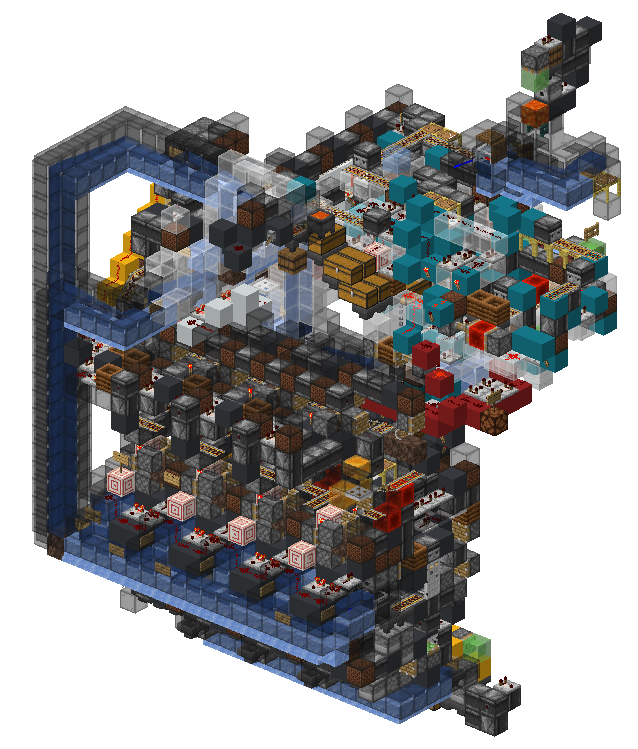
\includegraphics[width=0.48\textwidth]{asdadad.png}
    \caption{\centering High Speed Cart Based Ideal Splitter}
\end{figure}

% For wide tables, a single column layout is better. It can be switched
% page-by-page.
\onecolumn

\section{Device Specifications}

\begin{table}[h]
    \caption{Inputs}
    \begin{tabularx}{\textwidth}{l | c | X}
        \thickhline
        \textbf{Name} & \textbf{Range} & \textbf{Description} \\
        \hline
        Mixed boxes input & Box & Boxes to split. Boxes can contain any items. \\
        \thickhline
\end{tabularx}
\end{table}

\begin{table}[h]
    \caption{Outputs}
    \begin{tabularx}{\textwidth}{l | c | X}
        \thickhline
        \textbf{Name} & \textbf{Range} & \textbf{Description} \\
        \hline
        Split boxes output & Box & Boxes with same item types only \\
        \hline
        Unstackables output & Item & Unstackable items \\
        \thickhline
\end{tabularx}
\end{table}

\begin{table}[h]
    \caption{Device Specifications}
    \begin{tabularx}{\textwidth}{l | c c c | c | X}
        \thickhline
        \textbf{Parameter} & \textbf{Min.} & \textbf{Typ.} & \textbf{Max.} &
        \textbf{Unit} & \textbf{Conditions} \\
        \hline
        Throughput  & 0.5 & 20 & 31.5 & HS & Typical throughput includes item refresh downtime. \\
        \hline
        Active Lag & +2 & +10 & +16 & ms & At max speed with 4k item entities. Ryzen 5 3600, 2GB RAM. MC 1.19.3 with Lithium. \\
        \hline
        MC Version & 1.19 & 1.19.3 & - & MCV & Latest version at time of writing: 1.20.4\\
        \hline
        Dimensions & & 26 x 31 x 22 & & Blocks & \\
        \thickhline
\end{tabularx}
\end{table}

\newpage
\section{Testing Data}
\begin{table}[h]
\caption{Executed Tests}
\begin{tabularx}{\textwidth}{l | X}
    \thickhline
    \textbf{Test} & \textbf{Result} \\
    \hline
    Ideal splitting test & Device was able to split HermitCraft boxes correctly with minimum partial boxes. \\
    \thickhline
\end{tabularx}
\end{table}

\section{Download Information}
\begin{table}[h]
    \caption{Download Information}
    \begin{tabularx}{\textwidth}{l | l | l | X}
        \thickhline
        \textbf{Identifier} & \textbf{MC} & \textbf{File} & \textbf{Description} \\
        \hline
        SG03 & 1.19.3 & \href{https://github.com/Soontech-Annals/Archive/blob/8413f90a054b6c415703bae02badeba7541344f6/Archive/splitting/SG03\%20High\%20Speed\%20Cart\%20Based\%20Ideal\%20Splitter/SG03\_High\_Speed\_Cart\_Based\_Ideal\_Splitter.zip?raw=1}{SG03\_High\_Speed\_Cart\_Based\_Ideal\_Splitter.zip} & WDL of device. Cart unloader version included. Inventories included. \\
        \hline
        \thickhline
    \end{tabularx}
\end{table}

\newpage
\begin{sidewaysfigure}[h]
    \includegraphics[width=1\textwidth]{IdealSplitting3.png}
    \caption{\centering Logic Diagram of SG03 Ideal Splitter}
\end{sidewaysfigure}

\end{document}

